% WBR perception teaching deck -- Revision 2 facts and small fixes.
% Build: latexmk -xelatex main.tex   (see README.md)
% Content source: docs/SLIDES_OVERVIEW.md, docs/SYSTEM_GUIDE.md, docs/research/.
% Number policy: every number is a DESIGN value, a CALCULATED value, a HOST-TEST
% result, PUBLISHED figure, or explicitly sourced Pi MEASUREMENT; no STM32 measurement.
\documentclass[aspectratio=169,12pt,t]{beamer}

% Speaker notes: uncomment ONE line to see them.
% \setbeameroption{show notes on second screen=right}  % dual-screen (pdfpc)
% \setbeameroption{show only notes}                     % notes handout

\usetheme[progressbar=none, sectionpage=none]{moloch}
% A 208 x 117 mm canvas retains 16:9 and the actual 12pt class fonts.
% Long owner-approved sentences fit without frame scaling or reduced fonts.
\geometry{paperwidth=208mm,paperheight=117mm}

% ---------- fonts ----------
\usepackage{fontspec}
\setsansfont{Avenir Next}[BoldFont={Avenir Next Demi Bold}]
\setmonofont{Menlo}[Scale=1.0]
\newcommand{\captiontype}{\small}

% ---------- palette ----------
\definecolor{navy}{HTML}{1F3A5F}
\definecolor{teal}{HTML}{2A9D8F}
\definecolor{fault}{HTML}{E76F51}
\definecolor{paper}{HTML}{FAFAF7}
\definecolor{ink}{HTML}{22262B}
\definecolor{muted}{HTML}{6B7280}
\definecolor{rule}{HTML}{D6D9DE}

\setbeamercolor{normal text}{fg=ink, bg=paper}
\setbeamercolor{frametitle}{fg=paper, bg=navy}
\setbeamercolor{progress bar}{fg=teal, bg=rule}
\setbeamercolor{alerted text}{fg=fault}
\setbeamercolor{example text}{fg=teal}
\setbeamercolor{structure}{fg=navy}
\setbeamercolor{title separator}{fg=teal}
\setbeamercolor{footline}{fg=muted}
% Beamer otherwise inherits the fault/alert color for in-slide citations.
\setbeamercolor{bibliography entry author}{fg=navy}
\setbeamercolor{bibliography entry title}{fg=ink}
\setbeamercolor{bibliography entry location}{fg=muted}
\setbeamercolor{bibliography entry note}{fg=muted}
\setbeamercolor{block title}{fg=paper, bg=navy}
\setbeamercolor{block body}{bg=navy!6}
\setbeamerfont{frametitle}{size=\large, series=\bfseries}
\setbeamertemplate{frametitle}{\nointerlineskip\begin{beamercolorbox}[wd=\paperwidth,sep=2mm,leftskip=4mm]{frametitle}\usebeamerfont{frametitle}\insertframetitle\strut\end{beamercolorbox}}
\setbeamertemplate{itemize items}{\color{teal}\rule[0.25ex]{0.45em}{0.45em}}
\setbeamertemplate{bibliography item}[text]
\setbeamertemplate{page number in head/foot}[totalframenumber]
\hypersetup{colorlinks=true, linkcolor=navy, urlcolor=navy, citecolor=navy}
% Keep the appendix bookmark free of Beamer translation commands.
\pdfstringdefDisableCommands{\def\translate#1{#1}}

\setbeamertemplate{itemize subitem}{\color{muted}--}

% ---------- packages ----------
\usepackage{tikz}
\usetikzlibrary{arrows.meta, positioning, automata, calc, shapes.geometric, fit, backgrounds, decorations.pathreplacing}
\usepackage{booktabs}
\usepackage{array}
\newcolumntype{L}[1]{>{\raggedright\arraybackslash}p{#1}}
\usepackage{amsmath}
\usepackage{siunitx}
\sisetup{detect-all}

% ---------- helpers ----------
\newcommand{\muted}[1]{{\color{muted}#1}}

% \slideimg[<max height>]{<width>}{<V-id>}{<caption for placeholder>}
% Shows images/<V-id>.jpg or .png if present, otherwise a labelled gray box of the same size.
\newcommand{\slideimg}[4][0.64\textheight]{%
  \IfFileExists{images/#3.jpg}{%
    \includegraphics[width=#2, height=#1, keepaspectratio]{images/#3.jpg}%
  }{\IfFileExists{images/#3.png}{%
    \includegraphics[width=#2, height=#1, keepaspectratio]{images/#3.png}%
  }{%
    \begin{tikzpicture}
      \node[draw=rule, fill=black!6, rounded corners=2pt, minimum width=\dimexpr#2-1pt\relax, outer sep=0pt,
            minimum height=#1, align=center, text width=\dimexpr#2-8mm\relax, font=\small, text=muted]
        {\textbf{#3}\\[2pt]#4\\[2pt]\small Illustration pending};
    \end{tikzpicture}%
  }}%
}

\tikzset{
  box/.style={draw=navy, fill=white, rounded corners=2pt, align=center, font=\small,
              minimum height=7mm, inner sep=3pt},
  flow/.style={-{Stealth[length=2mm]}, thick, color=navy},
  faultflow/.style={-{Stealth[length=2mm]}, thick, color=fault},
  lbl/.style={font=\small, color=ink, fill=paper, inner sep=1pt},
}

% Only the page number appears in the footer.
\setbeamerfont{footline}{size=\small}
\setbeamertemplate{footline}{\hbox{\begin{beamercolorbox}[wd=\paperwidth,ht=4mm,dp=1mm,rightskip=6mm]{footline}\hfill\insertframenumber/\inserttotalframenumber\end{beamercolorbox}}}
\AtBeginSection{\begin{frame}[c]\centering{\Huge\bfseries\color{navy}\thesection. \insertsectionhead\par}\end{frame}}
\setbeamertemplate{navigation symbols}{}
\setbeamersize{text margin left=6mm,text margin right=6mm}
\setlength{\tabcolsep}{4pt}
\renewcommand{\arraystretch}{1.02}

\setlength{\emergencystretch}{2em}
\linespread{1.12}
\newcommand{\para}[1]{#1\par\medskip}
\newcommand{\lesson}[1]{\vfill{\color{teal!70!black}\bfseries #1}\par}
\newcommand{\illustration}[2]{\begin{center}\includegraphics[width=.86\linewidth,height=.38\textheight,keepaspectratio]{images/#1.png}\par\small\color{muted}#2\end{center}}
\newcommand{\twocol}[2]{\begin{columns}[T,onlytextwidth]\begin{column}{.48\textwidth}#1\end{column}\begin{column}{.48\textwidth}#2\end{column}\end{columns}}
\newcommand{\diagram}[1]{\begin{center}\begin{tikzpicture}[font=\normalsize]#1\end{tikzpicture}\end{center}}
\tikzset{word/.style={align=center,text width=32mm,minimum height=12mm,draw=rule,fill=white,rounded corners=2pt},dot/.style={circle,fill=teal,inner sep=2.5pt}}
\begin{document}\raggedright
\begin{frame}{How WBR perception works}

\para{A wheel-biped robot balances on two wheels at the ends of articulated legs. It needs to understand its motion while its controller keeps it upright.}
\illustration{P03}{Conceptual illustration: follow one camera moment through the system.}
\lesson{From sampled signals to an estimate of motion, then to a fair test.}

\note{Sources: \detokenize{slides_course/main.tex}. Teaching deck for a fourth-year electronics student. All reused illustrations are conceptual, not experimental evidence. WBR means wheel-biped robot.}
\end{frame}

\begin{frame}{We will follow one measurement from sensor to score}

\para{Imagine the robot turning past a table. The camera takes a left and right image of the same corner. Its motion sensor takes samples between images.}
\diagram{\foreach \x/\name/\txt in {0/a/Sensors,4.7/b/Time and space,9.4/c/Motion estimate,14.1/d/Fair test}{\node[word] (\name) at (\x,0){\txt};}\draw[flow](a)--(b);\draw[flow](b)--(c);\draw[flow](c)--(d);}
\para{First we learn what the signals mean. Then we learn how software combines them, how to judge the answer, and why the project tests each layer in order.}
{\small\muted{Reading map: sensors, pages 6--12; projector detail, 9--11; gate learning checklist, 44--45; appendix, 46--49.}\par}
\lesson{The same table corner will return throughout the deck.}

\note{Sources: \detokenize{slides_course/main.tex}. }
\end{frame}

\begin{frame}{The robot needs both its own motion and nearby geometry}

\para{Wheel rotation alone can mislead us when a wheel slips. A camera can see the table corner move across its image even when wheel measurements are wrong.}
\para{A \textbf{pose} is a position and an orientation: where the sensor is, and which way it points. A sequence of poses is a \textbf{trajectory}, or path through time.}
\para{Depth tells us how far away a visible surface is. Together, motion and depth help the robot reason about obstacles and where it can move.}
\lesson{Seeing a table is useful only if we know where the camera was when it saw it.}

\note{Sources: \detokenize{slides_course/main.tex}. }
\end{frame}

\begin{frame}{Balance must survive a delayed perception computer}

\twocol{\para{The \textbf{STM32H7} owns motor safety and the hard real-time control loop. Hard real-time means a deadline must be met to preserve the required behavior.}
\para{Think of a timer interrupt that must update control before the next tick.}}{\para{The \textbf{Raspberry Pi} runs perception on Linux. Image processing can take variable time, and the operating system can delay a task.}
\para{Its estimates must be checked for freshness and validity before a future controller interface uses them.}}
\diagram{\node[word] (p) at (0,0){Pi estimates motion};\node[word] (s) at (7,0){STM32H7 keeps control};\draw[flow,dashed](p)--node[above=8mm]{Planned checked interface}(s);}
\lesson{An old or missing pose must not become an unsafe motor command.}

\note{Sources: \detokenize{slides_progress/main.tex; AGENTS.md}. Existing ownership boundary only. No new interface, rate or fallback budget is proposed.}
\end{frame}

\begin{frame}{You can now explain why perception and control are separate}
\para{You should now be able to explain the following in your own words.}
\begin{itemize}
\item A pose describes position and orientation; depth describes distance to a surface.
\item The Pi can help understand the scene while the STM32H7 keeps responsibility for control and safety.
\item Explain what could happen if a controller treated an old pose as a current measurement.
\end{itemize}
\lesson{Try answering aloud before you turn the page.}
\note{Sources: \detokenize{slides_course/main.tex}. }
\end{frame}

\begin{frame}{The D435i combines two views with a motion sensor}

\illustration{P04}{Stylized D435i housing; the aperture drawing is not a hardware guide.}
\para{Two \textbf{infrared cameras} form a stereo pair: left and right views from different positions. The \textbf{IMU}, or inertial measurement unit, contains a gyroscope and an accelerometer.}
\para{In our running moment, both images see the table corner. The IMU measures the camera's turning and acceleration between image times.}
\lesson{The images and IMU provide different kinds of information about the same motion.}

\note{Sources: \detokenize{experiments/2026-10-13-SESSION_FACTS_FOR_SLIDES.md; slides_course/main.tex}. }
\end{frame}

\begin{frame}{Stereo depth comes from a corner shifting between views}

\para{\textbf{Disparity} is the horizontal difference between the positions of the same point in the left and right images. Nearby points shift more than distant points.}
\diagram{\draw[navy,thick](0,0)rectangle(5,1.7);\draw[navy,thick](8,0)rectangle(13,1.7);\node at(2.5,2.15){Left image};\node at(10.5,2.15){Right image};\node[dot](a)at(3,1){};\node[dot](b)at(10.4,1){};\draw[flow](a)--++(0,-1.5);\draw[flow](b)--++(0,-1.5);\node at(2.5,-.95){Corner at 120 pixels};\node at(10.5,-.95){Corner at 100 pixels};}
\para{Illustrative example: rectification aligns matching image rows. Focal length sets the projection scale in pixels. With $f=400$ pixels and camera separation $b=0.05$ metres, disparity $d=20$ pixels gives depth $Z=fb/d=1$ metre.}
\lesson{At 10 pixels of disparity, the same example gives 2 metres of depth.}

\note{Sources: \detokenize{slides_course/main.tex}. All numbers on this page are illustrative, not D435i calibration. Rectification digitally aligns the stereo views using calibration. Pinhole stereo geometry; focal length is defined here as projection scale in pixels and developed on calibration page.}
\end{frame}

\begin{frame}{IMU readings are useful signals with noise and bias}

\para{A \textbf{gyroscope} measures angular velocity: how fast the camera turns. An \textbf{accelerometer} measures specific force: acceleration relative to free fall. At rest on a table it reads about one g upward; in free fall it reads near zero. Here g is gravitational acceleration.}
\twocol{\para{\textbf{Noise} is the rapid random variation, like ADC readings that scatter around a steady input.}\para{\textbf{Bias} is an offset that may change slowly, like an ADC zero error.}}{\diagram{\draw[flow](0,0)--(5,0)node[right]{Time};\draw[navy,dashed](0,.8)--(5,.8);\node[below=1mm,font=\small]at(2.5,.8){Unbiased reference};\draw[teal,thick](0,1.3)--(.6,1.5)--(1.1,1.2)--(1.7,1.45)--(2.3,1.25)--(3,1.5)--(3.6,1.3)--(4.3,1.4)--(5,1.25);\node at(2.5,2){Offset plus scatter};\node at(2.5,-.6){Illustrative stationary signal};}}
\lesson{A gyro bias adds a little false rotation at every time step, so the angle error grows.}

\note{Sources: \detokenize{slides_course/main.tex}. }
\end{frame}

\begin{frame}{The projector is off so features belong to the room}

\para{A \textbf{feature} is a recognizable image detail, such as a corner. The infrared projector adds dots that can help the depth system match points on a plain surface.}
\diagram{\node[word] (a)at(0,0){Projected dots};\node[word] (b)at(6,0){Real table corner};\node[word] (c)at(12,0){Stable scene structure};\draw[faultflow,dashed](a)--++(0,-1.5)node[below,align=center]{Pattern can move\\with the projector};\draw[flow](b)--(c);}
\para{For visual motion estimation, we want persistent details attached to the room. Projected dots can change on surfaces as the camera moves and create misleading matches.}
\lesson{Turning off the projector trades artificial texture for more trustworthy natural texture.}

\note{Sources: \detokenize{experiments/2026-10-13-SESSION_FACTS_FOR_SLIDES.md; slides_progress/main.tex}. }
\end{frame}

\begin{frame}{The projector gives a plain wall texture for stereo depth}

\para{The D435i has a left infrared (IR) camera, a right IR camera and an IR projector. The cameras capture images; the projector produces no image. It shines an invisible dot pattern onto surfaces.}
\diagram{
  \node at (3,2.05) {White wall with projector OFF};
  \node at (12,2.05) {White wall with projector ON};
  \draw[navy,thick,fill=white] (0,0) rectangle (6,1.65);
  \draw[navy,thick,fill=white] (9,0) rectangle (15,1.65);
  \foreach \x/\y in {.4/.4,1.1/1.2,1.7/.65,2.5/1.35,3/.35,3.6/.95,4.2/1.4,4.7/.55,5.5/1.1,2.1/.2,5.7/.25,3.3/1.5}{
    \fill[teal] (9+\x,\y) circle (.055);
  }
  \node[font=\small] at (3,-.45) {No distinctive detail to match.};
  \node[font=\small] at (12,-.45) {Both IR cameras see added detail.};
}
{\small\muted{Illustrative IR views: the dots are invisible to our eyes.}\par}\medskip
\para{A plain wall can make left--right matching fail. Dots can make matching possible within the same stereo pair. For rectified images, disparity $d$ is the horizontal pixel shift of a matched point.}
\para{Depth is $Z=f\,b/d$: $f$ is focal length in pixels; $b$ is the distance between cameras (about 5 cm in our unit's nominal config); $d$ is disparity in pixels. $Z$ uses the same length unit as $b$.}
\lesson{Dots help identify a match; camera geometry turns its pixel shift into depth.}
\note{Sources: \detokenize{slides_learn/BRIEF.md Revision 4; experiments/2026-10-13-SESSION_FACTS_FOR_SLIDES.md section F; slides_course/main.tex}. Unit config baseline 0.0499 m is nominal factory geometry, not newly measured calibration. General active-stereo facts verified against RealSense, Projectors for D400 Series Depth Cameras, sections 1 and 3: https://dev.realsenseai.com/docs/projectors/ (accessed 14 October 2026). Schematic dots, not captured data or the actual projector pattern. Rectification was introduced on page 7. Stereo matches simultaneous views and does not require a pattern to remain fixed in the world across time.}
\end{frame}

\begin{frame}{A projected dot can slide while a real corner stays fixed}

ORB-SLAM3 estimates motion from fixed room features. A sliding dot can give wrong motion. Here the camera moves right above a flat table without turning.\par
{\centering
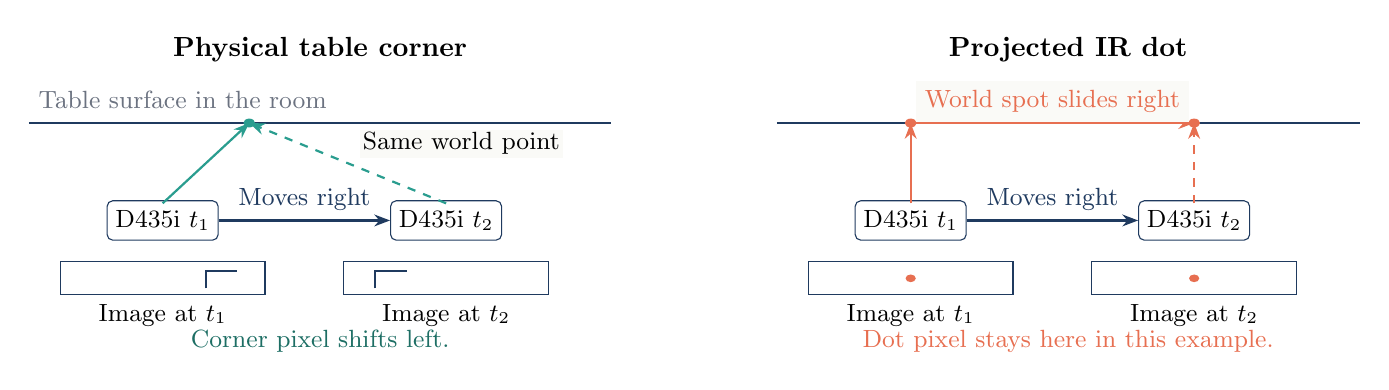
\begin{tikzpicture}[font=\small,y=.75cm]
\foreach \offset/\title in {0/Physical table corner,9.5/Projected IR dot}{
  \begin{scope}[xshift=\offset cm]
  \node[font=\normalsize\bfseries] at (4,3.55) {\title};
  \draw[navy,thick] (.3,2.3)--(7.7,2.3);

  \node[box,minimum height=5mm,font=\small] (c1) at (2,.65) {D435i $t_1$};
  \node[box,minimum height=5mm,font=\small] (c2) at (5.6,.65) {D435i $t_2$};
  \draw[flow] (c1.east)--node[above]{Moves right}(c2.west);
  \draw[navy] (.7,-.6) rectangle (3.3,-.05);
  \draw[navy] (4.3,-.6) rectangle (6.9,-.05);
  \node at (2,-.95) {Image at $t_1$};
  \node at (5.6,-.95) {Image at $t_2$};
  \end{scope}
}
\node[anchor=west,text=muted] at (.3,2.7) {Table surface in the room};
% Fixed corner: the later viewing ray leans left; its pixel shifts left.
\fill[teal] (3.1,2.3) circle (.075);
\node[anchor=west,fill=paper,inner sep=1pt] at (4.5,1.95) {Same world point};
\draw[flow,teal] (2,.94)--(3.1,2.3);
\draw[flow,teal,dashed] (5.6,.94)--(3.1,2.3);
\draw[navy,thick] (2.55,-.5)--(2.55,-.2)--(2.95,-.2);
\draw[navy,thick] (4.7,-.5)--(4.7,-.2)--(5.1,-.2);
\node[text=teal!70!black] at (4,-1.4) {Corner pixel shifts left.};
% The same projector ray moves with the rigid camera/projector assembly.
\fill[fault] (11.5,2.3) circle (.075);
\fill[fault] (15.1,2.3) circle (.075);
\draw[faultflow] (11.5,2.3)--node[above,fill=paper]{World spot slides right}(15.1,2.3);
\draw[flow,fault] (11.5,.94)--(11.5,2.3);
\draw[flow,fault,dashed] (15.1,.94)--(15.1,2.3);
\fill[fault] (11.5,-.33) circle (.065);
\fill[fault] (15.1,-.33) circle (.065);
\node[text=fault] at (13.5,-1.4) {Dot pixel stays here in this example.};
\end{tikzpicture}
\par}
{\small
\begin{tabular}{@{}L{.56\textwidth}L{.40\textwidth}@{}}
\toprule
Stereo depth on textureless surfaces & Often helpful.\\
ORB-SLAM3 feature tracking across time & Potentially misleading.\\
Our first natural-feature SLAM tests & OFF.\\\bottomrule
\end{tabular}\par\smallskip
The attached projector pattern follows the camera; its lit spots slide in the room. OFF is experimental: later compare ON and OFF for tracking quality and depth.\par}
\lesson{If the D435i moves right, does the table corner move in the room, or only in the image?}
\note{Sources: \detokenize{slides_learn/BRIEF.md Revision 4; experiments/2026-10-13-SESSION_FACTS_FOR_SLIDES.md; slides_progress/main.tex; slides_course/main.tex}. ORB-SLAM3 static-scene feature geometry: Campos et al. 2021, already linked on references page. Diagram is a geometric teaching example, not measured failure evidence: camera translates parallel to a flat table surface without rotating; one fixed projector ray intersects successive world points, while its image position remains constant for unchanged depth and rigid camera-projector geometry. General surfaces and rotations can change dot image positions too; camera-fixed emission directions do not mean every dot pixel is constant. Solid rays show t1, dashed rays t2. The corner does not move in the room; only its image position changes. Distinguish correspondence within one stereo pair from feature identity across time. OFF is this project's initial experimental choice, not a universal SLAM rule, and no ON/OFF comparison was run.}
\end{frame}

\begin{frame}{You can now explain what each sensor contributes}
\para{You should now be able to explain the following in your own words.}
\begin{itemize}
\item Two views turn a pixel shift into depth when camera geometry is known.
\item The gyro measures turning, and the accelerometer responds to motion and gravity.
\item Explain why random noise, slowly changing bias and moving projected dots cause different problems.
\end{itemize}
\lesson{Try answering aloud before you turn the page.}
\note{Sources: \detokenize{slides_course/main.tex}. }
\end{frame}

\begin{frame}{A coordinate frame says what a position is relative to}

\para{A \textbf{coordinate frame} is an origin and a set of axes. The same table corner has different coordinates relative to the camera, robot torso and room.}
\twocol{\diagram{\draw[navy,thick,rounded corners](1,1.7)rectangle(3,3);\draw[navy,very thick](1.4,1.7)--(.9,.9)--(1.3,0);\draw[navy,very thick](2.6,1.7)--(3.3,.9)--(3,0);\draw[navy,thick](1.3,-.3)circle(.3);\draw[navy,thick](3,-.3)circle(.3);\draw[flow,teal](2,2.3)--(4.4,2.3)node[right]{Body};\draw[flow,teal](2,2.3)--(2,4);\draw[flow,fault](2.7,3.1)--(4.3,3.7)node[right]{Camera};\draw[flow,fault](2.7,3.1)--(2.3,4.2);\draw[flow](0,-1)--(4,-1)node[right]{World};\draw[flow](0,-1)--(0,2);}}{\para{A \textbf{transform} converts coordinates between frames by rotating the axes and shifting the origin.}\para{Illustrative example: if the camera is 0.2 m ahead of the torso and their axes agree, a corner 1.0 m ahead of the camera is 1.2 m ahead of the torso.}\para{This schematic wheel-biped drawing shows two axes per frame to keep the geometry readable.}}
\lesson{Never compare positions until they describe the same frame.}

\note{Sources: \detokenize{slides_course/main.tex}. Schematic wheel-biped with torso, two articulated legs and one wheel at each foot. Axis directions are illustrative, not a proposed physical mounting convention.}
\end{frame}

\begin{frame}{A timestamp names the measurement time, not its arrival}

\para{A \textbf{timestamp} is a clock reading attached to a measurement. Like capturing a timer value at an interrupt, it tells us when the event happened.}
\diagram{\draw[flow](0,0)--(15,0)node[right]{Time};\foreach \x/\text in {1/Image exposure,6/USB delivery,11/Software reads}{\draw[navy,thick](\x,-.2)--(\x,.4);\node[align=center,text width=35mm]at(\x,1.1){\text};}\draw[teal,thick,<->](1,-1)--(6,-1)node[midway,below]{Transport delay};}
\para{Our stereo pair belongs at its exposure time. Motion samples must cover the interval since the previous image, even if the Pi receives some of them later.}
\lesson{Using arrival time would turn scheduling delays into apparent sensor motion.}

\note{Sources: \detokenize{docs/D435I_VIO_CALIBRATION_READINESS.md; slides_course/main.tex}. }
\end{frame}

\begin{frame}{Different clocks need a measured relationship}

\para{A \textbf{clock domain} is the time reference used by a clock. The camera, Pi and STM32 can each start counting at a different origin and run at slightly different rates.}
\diagram{\foreach \y/\name/\txt in {2/Camera/12.000 seconds,0/Pi/450.015 seconds,-2/STM32/8.002 seconds}{\node[anchor=east]at(0,\y){\name};\draw[flow](.5,\y)--(10,\y);\node[fill=paper]at(5,\y){\txt};}\draw[teal,dashed,thick](8,-2.4)--(8,2.4);\node[anchor=west]at(10.5,0){Same event};}
\para{Illustrative example: for this event, Pi time equals camera time plus 438.015 s. This \textbf{offset} relates their origins. If their rates differ, the offset changes; one paired reading cannot measure that drift.}
\lesson{Record the clock domain as carefully as the timestamp value.}

\note{Sources: \detokenize{docs/D435I_VIO_CALIBRATION_READINESS.md; slides_course/main.tex}. }
\end{frame}

\begin{frame}{You can now explain where and when a sample belongs}
\para{You should now be able to explain the following in your own words.}
\begin{itemize}
\item A frame names the axes and origin; a transform connects two frames.
\item A timestamp names a measurement event, while arrival time includes delivery delay.
\item Explain why subtracting two readings from unrelated clocks does not give a time delay.
\end{itemize}
\lesson{Try answering aloud before you turn the page.}
\note{Sources: \detokenize{slides_course/main.tex}. }
\end{frame}

\begin{frame}{Features let the computer recognize the same corner}

\para{A \textbf{feature} is a distinctive small image region, such as our table corner. ORB describes a region with bits from pixel-brightness comparisons. Think of a short binary signature for our corner.}
\diagram{\draw[navy,thick](0,0)rectangle(5,2.6);\draw[navy,thick](8,0)rectangle(13,2.6);\draw[navy,very thick](1,.5)--(1,1.8)--(3.5,1.8);\draw[navy,very thick](9,.5)--(9,1.8)--(11.5,1.8);\node[dot](a)at(1,1.8){};\node[dot](b)at(9,1.8){};\draw[flow,teal](a)--node[above,fill=paper]{Match}(b);\node at(2.5,-.5){One image};\node at(10.5,-.5){Another image};}
\para{\textbf{Feature matching} means deciding which regions show the same physical point. Similar signatures suggest a match. Many matches must also agree with one camera motion before software trusts them.}
\lesson{The table corner becomes a repeatable observation rather than a whole picture to memorize.}

\note{Sources: \detokenize{slides_course/main.tex}. ORB descriptor and geometric consistency: Campos et al. 2021. Drawing schematic, not measured feature output.}
\end{frame}

\begin{frame}{Tracking estimates the pose that explains the image}

\para{\textbf{Tracking} means estimating the current pose from recent measurements. If the camera turns, the table corner appears at a new pixel position.}
\diagram{\node[word](a)at(0,0){Earlier pose};\node[word](b)at(5,0){Predicted pose};\node[word](c)at(10,0){Image agrees?};\draw[flow](a)--(b);\draw[flow](b)--(c);\draw[flow,teal](c.south)--++(0,-1.2)-|node[below,pos=.25]{Correct the prediction}(b.south);}
\para{The estimator predicts where previously estimated scene points should appear, compares those predictions with observed pixels, and adjusts the pose to reduce the mismatch.}
\para{This resembles a control observer: predict the state, then use a measurement to correct it.}
\lesson{A pose is an estimate supported by many image matches, not a direct camera output.}

\note{Sources: \detokenize{slides_course/main.tex}. }
\end{frame}

\begin{frame}{Keyframes and map points preserve useful geometry}

\para{A \textbf{keyframe} is an image and its pose, kept because they add useful information. A \textbf{map point} is an estimated three-dimensional scene point observed in multiple images.}
\diagram{\foreach \x/\id/\txt in {0/a/First keyframe,6/b/New viewpoint,12/c/Later keyframe}{\node[word](\id)at(\x,0){\txt};}\node[dot](p)at(6,2.3){};\node[above]at(p){Table corner in the map};\draw[navy](a)--(p);\draw[navy](b)--(p);\draw[navy](c)--(p);}
\para{\textbf{SLAM} means simultaneous localization and mapping: estimating sensor poses and scene geometry together. Visual-inertial odometry estimates motion from images and IMU samples; SLAM also reuses a map and recognizes old places.}
\lesson{Stereo locates our corner in 3D; seeing it again helps locate the camera. Both estimates improve together.}

\note{Sources: \detokenize{slides_course/main.tex}. }
\end{frame}

\begin{frame}{The IMU predicts motion between camera images}

\para{Images arrive less often than IMU samples. \textbf{IMU preintegration} summarizes the turning and motion measured between two image times, instead of revisiting every sample for every pose correction.}
\diagram{\draw[flow](0,0)--(14,0);\foreach \x in {1,13}{\draw[navy,very thick](\x,-.3)--(\x,.6);}\foreach \x in {2,3,4,5,6,7,8,9,10,11,12}{\draw[teal,thick](\x,0)--(\x,.25);}\node at(1,1.2){Earlier image};\node at(13,1.2){Our stereo pair};\node at(7,-.8){Summarize the intervening IMU samples};}
\para{The IMU helps during rapid motion and helps estimate gravity. Stereo supplies distances in metres, rather than arbitrary units, through its known camera separation.}
\para{\textbf{IMU initialization} estimates starting velocity, gravity direction and sensor biases. Turning and accelerating in different directions help separate gravity from motion and sensor bias.}
\lesson{Images correct growing IMU motion error; this accumulated error is called drift.}

\note{Sources: \detokenize{slides_course/main.tex; experiments/2026-10-13-SESSION_FACTS_FOR_SLIDES.md}. Campos et al. 2021 visual-inertial initialization and preintegration. Timeline counts are schematic, not a requested sensor profile.}
\end{frame}

\begin{frame}{Three threads share the work and recognize old places}

\para{A \textbf{thread} is a software task that can run alongside other tasks. Our SLAM software, \textbf{ORB-SLAM3}, separates urgent tracking from slower map improvement and place recognition.}
\diagram{\node[word](a)at(0,0){Tracking\\Current pose};\node[word](b)at(6,0){Local mapping\\Refines the map};\node[word](c)at(12,0){Loop closing\\Recognizes places};\draw[flow](a)--(b);\draw[flow](b)--(c);\draw[flow,teal](c.south)--++(0,-1)-|(a.south);}
\para{\textbf{Loop closing} recognizes a place seen earlier. Returning to our table gives a new constraint: both visits should place the table at the same map location, so accumulated drift can be corrected.}
\lesson{Different responsibilities share one map; concurrent work does not guarantee a timing deadline.}

\note{Sources: \detokenize{slides_course/main.tex}. Campos et al. 2021 system overview. Diagram expresses conceptual data sharing, not an exhaustive thread synchronization graph.}
\end{frame}

\begin{frame}{Tracking fails when observations stop constraining motion}

\para{\textbf{Calibration} measures sensor properties so software can interpret the readings correctly.}
\begin{itemize}
\item Blur smears corners, and a blank wall offers few distinctive features to match.
\item Wrong calibration predicts the wrong pixels even for the correct pose.
\item Wrong time pairing combines an image with motion from a different instant.
\item A poorly initialized IMU can pull an otherwise plausible visual estimate in the wrong direction.
\end{itemize}
\para{In our running moment, a missed corner match is different from pairing the corner with the wrong turn. The symptom may look similar, but the layer to inspect is different.}
\lesson{Check input quality, time and geometry before changing algorithm settings.}

\note{Sources: \detokenize{slides_course/main.tex}. }
\end{frame}

\begin{frame}{You can now explain how images and IMU produce a pose}
\para{You should now be able to explain the following in your own words.}
\begin{itemize}
\item Features identify observations; tracking finds a pose that explains them.
\item Keyframes and map points preserve geometry, and loop closing constrains drift.
\item Explain how preintegration and initialization make IMU samples useful, and why bad inputs can still defeat SLAM.
\end{itemize}
\lesson{Try answering aloud before you turn the page.}
\note{Sources: \detokenize{slides_course/main.tex}. }
\end{frame}

\begin{frame}{Calibration tells software what the sensor geometry means}

\para{\textbf{Intrinsics} describe one camera's projection: focal length sets the pixel scale, the principal point is where the central viewing line of the camera meets the image, and distortion models lens warping.}
\para{\textbf{Extrinsics} describe the rotation and translation between sensors. Stereo needs the relation between cameras; visual-inertial estimation also needs the camera-to-IMU relation.}
\diagram{\node[word](a)at(0,0){Left camera};\node[word](b)at(6,0){Right camera};\node[word](c)at(12,0){IMU};\draw[flow,<->](a)--node[above=8mm]{Stereo geometry}(b);\draw[flow,<->](b)--node[above=8mm]{Rigid relation}(c);}
\lesson{Check that the sensor parameters describe this camera and predict its observed pixels correctly.}

\note{Sources: \detokenize{docs/D435I_VIO_CALIBRATION_READINESS.md; experiments/2026-10-13-SESSION_FACTS_FOR_SLIDES.md}. }
\end{frame}

\begin{frame}{Calibration must also describe time and uncertainty}

\twocol{\para{A \textbf{camera--IMU time offset} describes how far the image and motion timelines are shifted relative to each other. Sharing a clock domain alone does not establish their physical alignment.}\para{\textbf{IMU noise parameters} tell the estimator how much to trust samples and how quickly bias can change.}}{\illustration{P08}{Conceptual target; not a calibration grid.}}
\para{\textbf{Kalibr} fits camera and IMU geometry and timing from motion past a measured target. \textbf{Allan deviation} analyzes a long stationary IMU recording to estimate noise and slow bias behavior.}
\lesson{If IMU calibration is unavailable, assumed parameters still need measurement before we trust them.}

\note{Sources: \detokenize{docs/D435I_VIO_CALIBRATION_READINESS.md; experiments/2026-10-13-SESSION_FACTS_FOR_SLIDES.md}. Kalibr camera-IMU calibration and IMU noise model documentation. Current-unit factory warning is preserved in session facts; older-unit values must not be transferred.}
\end{frame}

\begin{frame}{You can now explain why calibration comes before trust}
\para{You should now be able to explain the following in your own words.}
\begin{itemize}
\item Intrinsics connect a three-dimensional point to a pixel, and extrinsics connect sensor frames.
\item Camera--IMU time offset and noise parameters describe different sources of error.
\item Explain why a room-motion test and a measured-target calibration recording answer different questions.
\end{itemize}
\lesson{Try answering aloud before you turn the page.}
\note{Sources: \detokenize{slides_course/main.tex}. }
\end{frame}

\begin{frame}{USB delivery and recording must keep up with the camera}

\para{The stereo pair and motion samples travel over local USB to the Pi. \textbf{librealsense} is the software development kit (\textbf{SDK}) that exposes images, motion readings and their metadata to programs.}
\para{A \textbf{buffer} temporarily holds data waiting to be written, like a UART receive queue. If the writer is slower than the arriving stream, the buffer fills and new frames are dropped.}
\diagram{\node[word](a)at(0,0){Camera samples};\node[word](b)at(6,0){Buffer fills};\node[word](c)at(12,0){Slow card writer};\draw[flow](a)--node[above=3mm,font=\small]{Data arrives}(b);\draw[faultflow](b)--node[above=3mm,font=\small]{Slow writing}(c);\draw[faultflow](b.south)--++(0,-.7)node[below,font=\small]{Full buffer drops frames};}
\para{Our 100-second take had long gaps. The card averaged 16.6 MB/s, below the 18.4 MB/s needed. A writer that could not keep up is the likely cause.}
\para{We now record short takes into Pi RAM, then copy to the card and verify the copy. A 15-second RAM test had no dropped frames. RAM is temporary: power loss can erase the take before copying.}
\lesson{Record locally on the Pi; a remote shell controls the session.}

\note{Sources: \detokenize{experiments/2026-10-14-SESSION_FACTS_ADDENDUM.md; slides_progress/main.tex; AGENTS.md}. Writer bottleneck is strongly inferred, not proven: first 100 s take had 0.3--2.9 s gaps after 22 s; 1.66 GB written; no under-voltage or USB errors in that take's kernel log. Short camera take delivered IR1/IR2 and IMU for 19 s with a shutdown gap. RAM test: 15 s, IR 29.99 Hz, max gap 33 ms, zero drops, gyro 200.2 Hz, accel 101 Hz; copied afterwards with checksum OK. RAM area 3.9 GB on 8 GB Pi; 100 s approximately 1.7 GB fits but sustained 100 s RAM capture is still untested in this addendum. RAM is volatile, not qualified permanent dataset storage. Acquisition remains local; SSH is control only.}
\end{frame}

\begin{frame}{ROS 2 messages make sensor data available to other tasks}

\para{\textbf{ROS 2} is robotics middleware: it connects software components. A \textbf{node} is a participating program; a \textbf{topic} is a named channel carrying a defined message type.}
\diagram{\node[word](a)at(0,0){Sensor node};\node[word](b)at(6,0){Image topic};\node[word](c)at(12,0){Recorder node};\draw[flow](a)--(b);\draw[flow](b)--(c);}
\para{The sensor node publishes each image; the recorder subscribes to receive it. The image message contains pixels and a header naming its time and coordinate frame. Other messages carry motion samples and calibration. Like a packet format, the metadata matters as much as the payload.}
\lesson{A topic name alone cannot prove that its messages have the right times or coordinate frames.}

\note{Sources: \detokenize{slides_course/main.tex; slides_progress/main.tex}. }
\end{frame}

\begin{frame}{Recording once lets us replay the same problem}

\para{A \textbf{bag} is a file-based recording of streams and their timing information. Replaying it lets us test identical input repeatedly, like saving a logic-analyzer trace instead of reproducing an intermittent interrupt.}
\twocol{\para{In the ROS 2 route, the driver publishes topics and rosbag2 records them. A separate input program must pass replayed images and IMU samples to SLAM.}\para{In the direct route, librealsense records the stereo pair and IMU samples. The D435i input program reads that recording and passes them to ORB-SLAM3.}}{\illustration{P10}{Conceptual review of recorded input.}}
\para{\textbf{Offline} processing reads saved input and can wait for computation. \textbf{Live} processing reads arriving samples and must keep up. A recording for one route may not be readable by the other.}
\lesson{Record first to separate input problems from live scheduling problems.}

\note{Sources: \detokenize{experiments/2026-10-13-SESSION_FACTS_FOR_SLIDES.md; slides_progress/main.tex}. SDK recording uses a rosbag2-format container in the installed SDK, but is not asserted interchangeable with the N3 ROS bag or Kalibr. Preserve source timestamps and input data.}
\end{frame}

\begin{frame}{You can now trace our moment through the software}
\para{You should now be able to explain the following in your own words.}
\begin{itemize}
\item The camera sends measurements over USB; librealsense exposes them to programs.
\item ROS 2 topics carry typed messages, and bags preserve input for repeated tests.
\item Explain how the ROS recording route differs from the direct librealsense input program, and what live processing adds.
\end{itemize}
\lesson{Try answering aloud before you turn the page.}
\note{Sources: \detokenize{slides_course/main.tex}. }
\end{frame}

\begin{frame}{Ground truth gives an independent answer to compare against}

\para{\textbf{Ground truth} is an independently measured reference, with its own uncertainty. A smooth estimated path is not enough: it can still be smoothly wrong.}
\para{\textbf{EuRoC} is a public drone dataset with stereo images, IMU samples and reference motion measurements. The machine-hall sequence called MH01 gives us known input before adapting to our camera.}
\diagram{\node[word](a)at(0,0){Recorded sensors};\node[word](b)at(6,0){Estimated pose};\node[word](c)at(12,0){Reference pose};\draw[flow](a)--(b);\draw[flow,<->,teal](b)--node[above=8mm]{Compare same time}(c);}
\lesson{Our table-camera recording needs an independent reference before we can claim absolute accuracy.}

\note{Sources: \detokenize{experiments/2026-10-13-SESSION_FACTS_FOR_SLIDES.md; slides_course/qa/n4a-traj-eval-summary.md}. Burri et al. 2016 EuRoC MAV datasets. Ground truth sources vary by sequence; MH01 uses the machine-hall position reference. Frame and clock assumptions are required before scoring.}
\end{frame}

\begin{frame}{Alignment removes an arbitrary origin without hiding scale}

\para{\textbf{Alignment} places two trajectories in the same coordinate frame. A \textbf{rigid alignment} rotates and shifts the entire estimated path once, without stretching it.}
\diagram{\draw[teal,very thick](0,0)--(2,0)--(2,2);\draw[fault,very thick](3,1)--(3,3)--(1,3);\node at(1.5,-.7){Before: different origins};\draw[flow](5,1)--(7,1);\draw[teal,very thick](9,0)--(11,0)--(11,2);\draw[fault,dashed,very thick](9,.12)--(11,.12)--(11.12,2);\node at(10,-.7){After: one shared frame};}
\para{Teal shows the reference; coral shows the estimate. SLAM can choose its own world origin, so removing that difference is fair. Stereo already provides distances in metres. Stretching its trajectory would conceal an error in those distances.}
\lesson{Match timestamps and sensor frames first; then use rotation and translation for the main score.}

\note{Sources: \detokenize{slides_course/qa/n4a-traj-eval-summary.md; slides_progress/main.tex}. Schematic paths; no measured results drawn. SE(3) alignment for main comparison, Sim(3) diagnostic only. Association tolerance 0.02 s; shared EuRoC clock assumed, zero offset; common IMU-body frame.}
\end{frame}

\begin{frame}{ATE measures the global position mismatch}

\para{\textbf{ATE}, absolute trajectory error, compares estimated and reference positions at matched times after alignment. A \textbf{residual} is one remaining difference.}
\twocol{\diagram{\draw[flow](0,0)--(5,0)node[right]{$x$};\draw[flow](0,0)--(0,3)node[above]{$y$};\node[dot](a)at(2,1){};\node[circle,fill=fault,inner sep=2.5pt](b)at(3.5,2){};\draw[thick,<->](a)--node[below right]{5 cm}(b);\node[below]at(a){Reference};\node[above]at(b){Estimate};}}{\para{Illustrative example: the aligned position differs by 3 cm in one direction and 4 cm in the perpendicular direction.}\para{The residual length is $\sqrt{3^2+4^2}=5$ cm.}\para{\textbf{RMSE}, root mean square error, squares every residual length, averages the squares, then takes the square root.}}
\lesson{ATE RMSE summarizes the whole matched path; it is not an error bound for every pose.}

\note{Sources: \detokenize{slides_course/qa/n4a-traj-eval-summary.md; slides_course/main.tex}. Example numbers illustrative. Diagram axes schematic, not to scale. For residuals 3 cm and 4 cm, RMSE would be sqrt((9+16)/2)=3.54 cm; example not included as experimental result.}
\end{frame}

\begin{frame}{RPE asks how much a short motion segment is wrong}

\para{\textbf{RPE}, relative pose error, compares motion between two times rather than absolute positions. It can measure both displacement error and turning error.}
\diagram{\draw[flow,teal](0,.6)--(9,.6);\draw[flow,fault](0,-.6)--(10,-.6);\node[anchor=east]at(0,.6){Reference};\node[anchor=east]at(0,-.6){Estimate};\node at(0,1.4){Start};\node at(9,1.4){One second later};\draw[thick,<->](9,-1.2)--(10,-1.2);\node[below]at(9.5,-1.2){1 cm difference};}
\para{Illustrative drawing, not to scale: reference displacement is 1.00 m, estimate is 1.01 m, with no turning difference. Translational RPE is 1 cm.}
\para{Our evaluation selects segments ending at least one second after their start. This describes local drift over that interval, not a constant error rate.}
\lesson{ATE asks about the global path; RPE asks about individual motion segments.}

\note{Sources: \detokenize{slides_course/qa/n4a-traj-eval-summary.md}. Pair policy: first later reference timestamp >= 1 s per eligible start, no interpolation. Actual rotational RMSE about 0.076 degrees. Arrows schematic, not to scale.}
\end{frame}

\begin{frame}{Three EuRoC runs support the build, not our camera}

\para{The input is about 184 seconds of drone motion. The evaluated reference span covers about 81 metres of travel. Each run uses the same recorded sensor data.}
\begin{center}\begin{tabular}{lrr}\toprule
 & Global ATE RMSE & One-second translational RPE RMSE\\\midrule
First run & 4.15 cm & 1.33 cm\\
Second run & 3.68 cm & 1.36 cm\\
Third run & 4.16 cm & 1.40 cm\\\bottomrule
\end{tabular}\end{center}
\para{The ORB-SLAM3 paper reports about 3.6 cm ATE on MH01. Our three-run average is about 4.0 cm. The paper reports the median of ten runs: the average of the two middle results when ordered. Evaluation details can differ, so this is only a rough comparison.}
\para{The runs show that our Pi executable estimates motion on known input. They do not test D435i calibration or healthy real-time speed; under-voltage affected the Pi.}

\note{Sources: \detokenize{experiments/2026-10-13-SESSION_FACTS_FOR_SLIDES.md; slides_course/qa/n4a-traj-eval-summary.md; slides_progress/main.tex}. Paper comparator verified in slides_progress: Campos et al. 2021 Table II, MH01 stereo-inertial 0.036 m; median of ten runs and processed GT. Local RPE independently calculated by trajectory_eval, not evo RPE. Evaluated matched span ~181.88 s and 80.606 m; full input ~184 s. All three one map, no resets, IMU initialized. Run times 301/282/284 s under power faults; no gate PASS inferred.}
\end{frame}

\begin{frame}{You can now explain what an accuracy score proves}
\para{You should now be able to explain the following in your own words.}
\begin{itemize}
\item Ground truth must independently measure the quantity we want to test.
\item Rigid alignment removes an arbitrary origin; ATE and RPE answer different questions.
\item Explain why good EuRoC accuracy does not qualify the D435i, its timing or live speed.
\end{itemize}
\lesson{Try answering aloud before you turn the page.}
\note{Sources: \detokenize{slides_course/main.tex}. }
\end{frame}

\begin{frame}{The first gates establish a trustworthy sensor path}

\para{A \textbf{gate} is a question that must be answered with evidence before depending on that layer. It is like checking power and UART framing before debugging the application protocol.}
\begin{itemize}
\item \textbf{N0 asks whether the Pi has stable power, cooling and a usable platform.} An unstable computer makes later failures ambiguous.
\item \textbf{N1 asks whether the intended camera has correct USB access.} Its own link must be at least 5000 megabits per second; a slow fallback can limit delivery.
\item \textbf{N2 asks whether raw samples, directly from the sensor, arrive correctly over time.} A mandatory 300-second continuous run (five minutes) catches sustained faults that a brief preview can miss.
\item \textbf{N3 asks whether ROS 2 preserves those measurements through recording and replay.} This isolates middleware faults before estimation.
\end{itemize}

\note{Sources: \detokenize{slides_progress/main.tex}. N2 exact baseline: IR1-only 640x480 Y8 at 15 Hz, gyro 200 Hz, accel 100 Hz; 20/105/300 s stages. Thresholds and profile remain unchanged in actual Phase A runbook. No command performed.}
\end{frame}

\begin{frame}{The estimation gates separate algorithm, camera and timing load}

\begin{itemize}
\item \textbf{N4A asks whether the build works on known EuRoC input.} It can be investigated independently of camera transport because the dataset already supplies measurements.
\item \textbf{N4B asks whether recorded D435i input supports reliable offline estimation.} First check sensor delivery, review adding the second camera stream, and check calibration. Then replay the same recording to investigate estimation.
\item \textbf{N4C asks whether live estimation keeps up without losing trustworthy input.} It comes after offline review because live scheduling adds another possible failure source.
\end{itemize}
\para{N2 checks one infrared stream. Stereo needs a second stream and more data delivery, so it needs an additional reviewed test. Passing N2 alone does not test stereo.}
\lesson{Offline replay lets us investigate estimation before adding live timing pressure.}

\note{Sources: \detokenize{slides_progress/main.tex; experiments/2026-10-13-SESSION_FACTS_FOR_SLIDES.md}. N4B development may expose calibration problems; repeat qualified offline review with accepted calibration before N4C. Main gate ladder is instructional, no authorization for execution.}
\end{frame}

\begin{frame}{The final gates connect timing evidence to safe use}

\begin{itemize}
\item \textbf{N5 asks where computation time and resources go.} Measure processing, queues and sample age before promising a usable update rate.
\item \textbf{N6 asks whether unreliable perception is detected and handled.} A pose can be old or invalid. If SLAM restarts its map, the world origin can change; the controller must detect that change before using the pose.
\item \textbf{N7 asks whether the controller integration behaves safely.} It follows timing and health checks because the STM32H7 must know when a perception input is usable.
\end{itemize}
\para{\textbf{Latency} is delay between defined events. \textbf{Sample age} is how old the measurement is when consumed. A short computation can still use old input if a queue is growing.}
\lesson{Define clock relationships and failure behavior before making a control promise.}

\note{Sources: \detokenize{slides_course/main.tex; slides_progress/main.tex}. N5/N6/N7 planned. Existing safety ownership preserved; no public interface or numeric budget introduced.}
\end{frame}

\begin{frame}{Debug from the physical layer upward}

\diagram{\foreach \x/\name/\txt in {0/a/Power,4.5/b/Raw input,9/c/Time and geometry,13.5/d/Estimator}{\node[word](\name)at(\x,0){\txt};}\draw[flow](a)--(b);\draw[flow](b)--(c);\draw[flow](c)--(d);}
\para{If raw samples already have gaps, changing SLAM parameters cannot recover missing measurements. If replay is good but live input falls behind, inspect scheduling and queues.}
\para{Our offline D435i program crashed on its first frame. A \textbf{pointer} stores an address, as in embedded C. ORB-SLAM3 checked an uninitialized keyframe pointer: it read a garbage value and tried to access that address before any keyframe existed.}
\para{The fix sets that pointer to null, meaning no keyframe yet, before the check. The EuRoC example never asked for this value. Power loss interrupted the rebuild, so a successful rerun is still needed to verify the fix.}
\lesson{The next investigation should answer the first unresolved question, not the most exciting one.}

\note{Sources: \detokenize{experiments/2026-10-14-SESSION_FACTS_ADDENDUM.md; slides_progress/main.tex; AGENTS.md}. First-frame SIGSEGV backtrace: main to System::GetTimeFromIMUInit to LocalMapping::GetCurrKFTime. Upstream LocalMapping::mpCurrentKeyFrame uninitialized; patch 4 sets KeyFrame* mpCurrentKeyFrame = nullptr in include/LocalMapping.h, committed in Pi build copy. EuRoC example does not call this function; N4A evidence unaffected. Rebuild interrupted by power loss after 3 of approximately 27 library objects; no successful patched rerun is reported. No upstream source or runtime changed by this deck revision. Preserve failure logs and change one cause at a time; offline investigation also checks image quality, timestamps, initialization and calibration.}
\end{frame}

\begin{frame}{You can now explain why the gates have this order}
\para{You should now be able to explain the following in your own words.}
\begin{itemize}
\item N0 through N3 check the computer and sensor delivery; N4 tests known recordings, our camera recordings and live estimation.
\item N5 through N7 check delays, detect unusable poses and test safe use by the controller.
\item Explain which layer you would inspect if replay succeeds while live tracking falls behind.
\end{itemize}
\lesson{Try answering aloud before you turn the page.}
\note{Sources: \detokenize{slides_course/main.tex}. }
\end{frame}

\begin{frame}{Today short camera tests work, but power still limits progress}

\para{As of 14 October 2026, the 8 GB Pi runs the same OS card. Both infrared views and IMU samples arrived during a short camera test. The three earlier EuRoC trajectories remain our known-input baseline.}
\para{The microSD and tested USB stick are too slow for recording. A short RAM recording worked, with a verified copy afterwards; the longer take still needs testing.}
\para{The offline camera program crashed. Its pointer fix is applied, but the rebuild was interrupted. Under-voltage persists on the same supply: more RAM did not fix power. These are diagnostic results, not completed gates.}
\para{Next: restore stable power and resume the rebuild, then test a 100-second RAM take and offline replay before a live demo. Calibration, qualified data storage and the required gate checks are still needed before trusting the system.}
\lesson{Camera tests require your explicit ``CAMERA AVAILABLE'' confirmation.}

\note{Sources: \detokenize{experiments/2026-10-14-SESSION_FACTS_ADDENDUM.md; experiments/2026-10-13-SESSION_FACTS_FOR_SLIDES.md; slides_progress/main.tex; AGENTS.md}. Single current-status page. Raspberry Pi 5 Rev 1.1, 7.8 GiB RAM with unchanged 32 GB OS card; under-voltage within 3 min on 5 V/3 A supply. Short 20 s camera take delivered 19 s with approximately 0.7 s shutdown gap; 15 s RAM test zero drops and checksum-verified copy. First 100 s card take unusable; 100 s RAM take planned. USB 2.0 stick 1.09 MB/s with fsync, data untouched. Patch applied in Pi build copy, rebuild interrupted, no successful offline D435i trajectory yet. Tomorrow's RAM/offline/live path is diagnostic and does not bypass N0--N3 or calibration; demos remain unaccepted until power and calibration exist. Wi-Fi on 8 GB Pi did not appear within approximately 7 min; cause unknown, current remote access not claimed. MicroSD is OS/tools/small logs; large bags require separately qualified storage. New camera identity differs from September unit; four serial-related fields remain distinct. No new capture, device access or ORB execution performed.}
\end{frame}

\begin{frame}{You can now choose and explain the next useful task}
\para{You should now be able to explain the following in your own words.}
\begin{itemize}
\item Tell the story of one stereo pair and its IMU samples from capture through recording to a pose and a score.
\item Explain what the EuRoC tests showed, what our camera still needs to prove, and why controller integration comes later.
\item For the next test, explain the question, the measurements needed, and which failure would make you stop.
\end{itemize}
\lesson{Try answering aloud before you turn the page.}
\note{Sources: \detokenize{slides_course/main.tex}. }
\end{frame}

\begin{frame}{What to learn before each gate}

{\small
\begin{tabular}{@{}L{45mm}L{47mm}L{43mm}L{51mm}@{}}\toprule
\textbf{Gate and its question} & \textbf{Concepts to understand first} & \textbf{One primary source to read} & \textbf{Self-check}\\\midrule
\textbf{N0.} Is the Pi stable under load? & Power and cooling; throttling means reduced processor speed. & Raspberry Pi hardware docs: power and cooling. & Why can low voltage make a speed test misleading?\\[4pt]
\textbf{N1.} Can we access the intended camera over fast USB? & Device identity; actual USB link speed; permissions. & librealsense troubleshooting guide: USB connection. & Why does a fast USB hub not prove the camera link is fast?\\[4pt]
\textbf{N2.} Do raw samples keep arriving correctly? & Sample intervals; gaps; bias; Allan analysis compares noise across averaging times. & Kalibr IMU noise model: Allan analysis. & Why does a short, clean preview not prove sustained delivery?\\[4pt]
\textbf{N3.} Does ROS 2 preserve data through recording and replay? & Topics; QoS means delivery rules; tf2 handles frame transforms; bag replay. & ROS 2 tutorials: topics, QoS, tf2 and recording. & What must survive replay besides the image pixels?\\\bottomrule
\end{tabular}}

\note{Sources: \detokenize{slides_learn/BRIEF.md Revision 3; slides_progress/main.tex; slides_course/main.tex; docs/PERCEPTION_TOOLING_ARCHITECTURE.md}. Primary readings: Raspberry Pi hardware documentation; librealsense Troubleshooting Q\&A; ETH ASL Kalibr IMU Noise Model; official ROS 2 Jazzy tutorials. Links on references page. N2 Allan reading explains sensor noise, not transport acceptance: sample gaps and intervals still need raw delivery evidence. The 300-second soak is not an Allan calibration record. N1 USB >=5000M on the camera's own branch; N2 exact IR1-only profile and 20/105/300-second sequence unchanged. Self-check answers: N0 reduced frequency or resets confound speed; N1 downstream link can fall back independently; N2 intermittent/sustained faults require full soak; N3 preserve timestamps, clock meaning, frames, camera geometry, IMU values and completeness. Eight rows with four columns require tiny text on one page; two pages retain readable type. Reading only; no gate acceptance or hardware action.}
\end{frame}

\begin{frame}{What to learn before each gate}

{\small
\begin{tabular}{@{}L{45mm}L{47mm}L{43mm}L{51mm}@{}}\toprule
\textbf{Gate and its question} & \textbf{Concepts to understand first} & \textbf{One primary source to read} & \textbf{Self-check}\\\midrule
\textbf{N4.} Can we estimate motion on known data, camera replay, then live input? & Features; calibration; IMU preintegration; ground truth; ATE and RPE. & Campos et al. (2021), ORB-SLAM3 paper. & Why does a good EuRoC score not qualify our camera or live speed?\\[4pt]
\textbf{N5.} Where do processing time and resources go? & Latency; queue growth; sample age; clock relationships; processor load. & ROS 2 tracing tutorial: measuring execution time. & How can fast processing still deliver an old pose?\\[4pt]
\textbf{N6.} Can we detect and handle an unusable pose? & Pose transforms in 3D; map resets; invalid or old measurements. & Barfoot, \emph{State Estimation for Robotics}: pose transforms. & Why must a new map origin be detected before using a pose?\\[4pt]
\textbf{N7.} Does controller integration behave safely? & Local deadlines; watchdog timeouts; fallback behavior. & STMicroelectronics STM32H7 independent watchdog training. & If the Pi stops sending poses, which safety loops must stay local?\\\bottomrule
\end{tabular}}

\note{Sources: \detokenize{slides_learn/BRIEF.md Revision 3; slides_progress/main.tex; slides_course/main.tex; docs/ORB_SLAM3_OFFLINE_PREPARATION.md; AGENTS.md}. Primary readings: Campos et al. 2021; official ROS 2 tracing tutorial; Barfoot State Estimation for Robotics second edition, pose/SE(3) material; ST STM32H7 independent watchdog training. N4 groups N4A EuRoC, N4B D435i offline and N4C live; N4A does not need camera acquisition. Supplementary calibration and evaluation readings on references page. N5 remains timing/resources, not trajectory evaluation. ROS tracing teaches callback duration, not automatically sensor-to-controller latency or direct-SDK timing. Barfoot teaches transforms, not a complete N6 health protocol. ST teaches watchdog mechanisms, not an approved safety procedure; MCU reset is not asserted to maintain balance. Self-check answers: N4 known recordings do not validate our hardware/calibration or live scheduling; N5 queues hold old input; N6 a changed origin invalidates consumer continuity assumptions; N7 body IMU, balance loop, motor limits and watchdog/fallback stay on STM32H7. No interface, message, safety policy, budget or runtime change.}
\end{frame}

\begin{frame}{These terms summarize the ideas you have learned}

\twocol{
\para{\textbf{Pose and trajectory.} Position plus orientation, and their history.}
\para{\textbf{Disparity.} A point's horizontal shift between stereo views.}
\para{\textbf{Feature and match.} A distinctive image region, and its correspondence.}
\para{\textbf{Keyframe and map point.} A kept image with its pose, and an estimated scene point.}
\para{\textbf{Bias.} A sensor offset that may slowly change.}
\para{\textbf{Preintegration.} A summary of IMU motion between image times.}
}{
\para{\textbf{Frame and transform.} Axes and origin, and a conversion between them.}
\para{\textbf{Timestamp and clock domain.} An event's time and its clock reference.}
\para{\textbf{Intrinsics and extrinsics.} Camera projection and relations between sensors.}
\para{\textbf{Alignment.} Placing paths in one frame.}
\para{\textbf{ATE and RPE.} Global position error and error in a motion segment.}
\para{\textbf{RMSE.} The square root of the average squared errors.}
}

\note{Sources: \detokenize{slides_course/main.tex}. }
\end{frame}

\begin{frame}{Each tool answers a different engineering question}

\begin{tabular}{@{}p{42mm}p{145mm}@{}}\toprule
\textbf{Tool} & \textbf{Purpose}\\\midrule
librealsense & Reads camera measurements and SDK recordings.\\[6pt]
realsense-ros & Publishes camera data and metadata as ROS 2 messages.\\[6pt]
rosbag2 & Records and replays ROS 2 topic streams.\\[6pt]
ORB-SLAM3 & Estimates poses and a map from images and motion samples.\\[6pt]
evo & Evaluates estimated trajectories against reference trajectories.\\[6pt]
Trajectory evaluator & Calculates the documented local RPE and comparison plots.\\[6pt]
Kalibr & Fits sensor geometry and time offset from a measured target.\\[6pt]
Allan analysis & Estimates noise and bias behavior from stationary IMU data.\\\bottomrule
\end{tabular}
\lesson{Choose the tool from the question you need to answer.}

\note{Sources: \detokenize{slides_progress/main.tex; docs/D435I_VIO_CALIBRATION_READINESS.md}. }
\end{frame}

\begin{frame}{Use these commands to rebuild the deck or score saved paths}

\para{Deck-only reproduction from this repository. These commands do not access the camera.}
{\small\ttfamily
cd slides\_learn\par
latexmk -xelatex -interaction=nonstopmode main.tex\par\medskip
swift -module-cache-path qa/swift-cache \textbackslash{}\par
\quad \textasciitilde/Desktop/OS/OS-project/heterogeneous-edge-ai-os/slides/render.swift \textbackslash{}\par
\quad main.pdf preview\par}
\medskip\para{Example command for scoring saved trajectories:}
{\small\ttfamily evo\_ape tum REFERENCE.tum ESTIMATE.tum -a\par}
\medskip\para{First make times, frames and file formats compatible. The alignment option rotates and shifts; it does not correct sensor timing or establish ground truth. Camera procedures stay in the approved runbook.}

\note{Sources: \detokenize{slides_progress/main.tex}. Command cheat-sheet includes actual deck reproduction and future evo shape from progress deck. Not executed here: trajectory scoring or physical sensor procedures. REFERENCE/ESTIMATE are placeholders; ORB output needs validated parsing/conversion.}
\end{frame}

\begin{frame}{The sources separate project evidence from general methods}

{\small
\textbf{Project evidence.} October 13 session facts and October 14 addendum; three-run evaluation; calibration notes; course, progress and report decks. Page notes hold detailed provenance.\par\medskip
\begin{columns}[T,onlytextwidth]
\begin{column}{.48\textwidth}
\textbf{Power and USB.} Raspberry Pi \href{https://www.raspberrypi.com/documentation/computers/raspberry-pi.html}{hardware docs}: power and cooling. RealSense \href{https://github.com/realsenseai/librealsense/wiki/Troubleshooting-Q\%26A}{librealsense troubleshooting}: USB access.\par\medskip
\textbf{ROS 2.} Official \href{https://docs.ros.org/en/jazzy/Tutorials.html}{Jazzy tutorials}: topics, QoS, tf2 and bags; \href{https://docs.ros.org/en/jazzy/Tutorials/Advanced/ROS2-Tracing-Trace-and-Analyze.html}{tracing tutorial}: execution time.\par\medskip
\textbf{SLAM and data.} Campos et al. (2021), \href{https://arxiv.org/abs/2007.11898}{ORB-SLAM3}, including Table II. Burri et al. (2016), \href{https://projects.asl.ethz.ch/datasets/doku.php?id=kmavvisualinertialdatasets}{EuRoC datasets}.\par\medskip
\textbf{Calibration and noise.} Furgale et al. (2013), \href{https://github.com/ethz-asl/kalibr/wiki}{Unified Temporal and Spatial Calibration}. Kalibr \href{https://github.com/ethz-asl/kalibr/wiki/camera-imu-calibration}{camera--IMU guide} and \href{https://github.com/ethz-asl/kalibr/wiki/IMU-Noise-Model}{IMU noise model}, including Allan analysis.\par
\end{column}
\begin{column}{.48\textwidth}
\textbf{Inertial estimation.} Forster et al. (2017), \href{https://arxiv.org/abs/1512.02363}{On-Manifold Preintegration for Real-Time Visual-Inertial Odometry}.\par\medskip
\textbf{Trajectory evaluation.} Sturm et al. (2012), \href{https://cvg.cit.tum.de/data/datasets/rgbd-dataset}{RGB-D SLAM benchmark}: ATE and RPE. Zhang and Scaramuzza (2018), \href{https://rpg.ifi.uzh.ch/docs/IROS18_Zhang.pdf}{quantitative trajectory evaluation tutorial}. Maintainer's \href{https://github.com/MichaelGrupp/evo/wiki/Metrics}{evo metric guide}.\par\medskip
\textbf{Frames and safe use.} Barfoot, \href{https://asrl.utias.utoronto.ca/~tdb/bib/barfoot_ser24.pdf}{State Estimation for Robotics}, second edition: 3D pose transforms, called SE(3). ST \href{https://www.st.com/content/st_com/en/support/learning/stm32-online-training/stm32h7-online-training.html}{STM32H7 watchdog training}.\par\medskip
\textbf{Projector.} RealSense, \href{https://dev.realsenseai.com/docs/projectors/}{Projectors for D400 Series}: texture for stereo depth.\par\smallskip
\textbf{Images.} Reused course illustrations are conceptual; new diagrams are schematic. Worked numbers are illustrative.\par
\end{column}
\end{columns}}
\note{Sources: \detokenize{experiments/2026-10-14-SESSION_FACTS_ADDENDUM.md; experiments/2026-10-13-SESSION_FACTS_FOR_SLIDES.md; slides_course/qa/n4a-traj-eval-summary.md; docs/D435I_VIO_CALIBRATION_READINESS.md; slides_course/main.tex; slides_progress/main.tex; slides_report/main.tex; slides_learn/BRIEF.md Revision 3}. Primary references checked 14 October 2026. Furgale, Rehder and Siegwart: Unified Temporal and Spatial Calibration for Multi-Sensor Systems, IROS 2013 (Kalibr bibliography). Forster, Carlone, Dellaert and Scaramuzza: IEEE Transactions on Robotics 2017; linked preprint submitted 2015. Sturm et al.: A Benchmark for the Evaluation of RGB-D SLAM Systems, IROS 2012. Zhang and Scaramuzza: A Tutorial on Quantitative Trajectory Evaluation for Visual(-Inertial) Odometry, IROS 2018. Barfoot second edition 2024; linked author's updated draft compiled September 2026. ROS docs web access blocked by Anubis; content verified against official ros2/ros2\_documentation jazzy source and ROS documentation mirror. ST training contains Independent watchdog (IWDG); this reading supplies mechanisms, not a WBR safety approval. Camera methods are background reading; no camera command authorized. Theme and assets unchanged. Sources are not gate acceptance.}
\end{frame}
\end{document}
